\documentclass[cjk,dvipdfmx,10pt,compress,%
hyperref={bookmarks=true,bookmarksnumbered=true,bookmarksopen=false,%
colorlinks=false,%
pdftitle={第 79 回 関西 Debian 勉強会},%
pdfauthor={倉敷・のがた・佐々木・かわだ・八津尾},%
%pdfinstitute={関西 Debian 勉強会},%
pdfsubject={資料},%
}]{beamer}

\title{第 79 回 関西 Debian 勉強会}
\subtitle{$\sim$発表資料$\sim$}
\author[かわだ てつたろう]{{\large\bf 倉敷・のがた・佐々木・かわだ・八津尾}}
\institute[Debian JP]{{\normalsize\tt 関西 Debian 勉強会}}
\date{{\small 2013 年 12 月 22 日}}

%\usepackage{amsmath}
%\usepackage{amssymb}
\usepackage{graphicx}
\usepackage{moreverb}
\usepackage[varg]{txfonts}
\AtBeginDvi{\special{pdf:tounicode EUC-UCS2}}
\usetheme{Kyoto}
\def\museincludegraphics{%
  \begingroup
  \catcode`\|=0
  \catcode`\\=12
  \catcode`\#=12
  \includegraphics[width=0.9\textwidth]}
%\renewcommand{\familydefault}{\sfdefault}
%\renewcommand{\kanjifamilydefault}{\sfdefault}
\begin{document}
\settitleslide
\begin{frame}
\titlepage
\end{frame}
\setdefaultslide

\begin{frame}[fragile]
\frametitle{Agenda}

\tableofcontents

\end{frame}

\section{最近の Debian 関係のイベント}

\takahashi[40]{最近の Debian\\関係のイベント}

\begin{frame}[fragile]
  \frametitle{第77回関西Debian勉強会}
  \begin{itemize}
  \item 日時: 10月27日(日)
  \item 場所: 港区民センター
  \end{itemize}
  \begin{block}{内容}
    \begin{itemize}
    \item 「ALSAのユーザランド解説」
    \item 「git-buildpackage入門again」
    \end{itemize}
  \end{block}
\end{frame}

\begin{frame}[fragile]
  \frametitle{第78回関西Debian勉強会@関西オープンソース2013}
  \begin{itemize}
  \item 日時: 11月9日(土)
  \item 場所: 大阪南港ATC
  \end{itemize}
  \begin{block}{内容}
    \begin{itemize}
    \item ブース展示
    \item セッション「Debian7.0の実情/今後の開発について」
    \end{itemize}
  \end{block}
\end{frame}

\begin{frame}[fragile]
  \frametitle{第106回東京エリアDebian勉強会}
  \begin{itemize}
  \item 日時: 11月16日(土)
  \item 場所: あんさんぶる荻窪
  \end{itemize}
  \begin{block}{内容}
    \begin{itemize}
    \item 「waylandを動かす」
    \item 「Emacs tramp(transparent remote file access)」
    \end{itemize}
  \end{block}
\end{frame}

\begin{frame}[fragile]
  \frametitle{第107回東京エリアDebian勉強会}
  \begin{itemize}
  \item 日時: 12月21日(土)
  \item 場所: あんさんぶる荻窪
  \end{itemize}
  \begin{block}{内容}
    \begin{itemize}
    \item 「debian GNU/Hurd」
    \item 「Debian勉強会2014年度計画」
    \end{itemize}
  \end{block}
\end{frame}

\begin{frame}[fragile]
  \frametitle{Debianもくもくの会}
  \begin{block}{第0回Debianもくもくの会}
    \begin{itemize}
    \item 日時: 11月23日(土)
    \item 場所: ミラクル・リナックス
    \end{itemize}
  \end{block}
  \begin{block}{第1回Debianもくもくの会}
    \begin{itemize}
    \item 日時: 12月14日(土)
    \item 場所: 朝日ネット
    \end{itemize}
  \end{block}
\end{frame}

\begin{frame}[fragile]
  \frametitle{Debian Project}
  \begin{itemize}
  \item 「Debian Policy 3.9.5.0 released」
  \item 「Alioth is down/alioth back online」
  \item 「Release sprint results - team changes, auto-rm and arch status」
  \end{itemize}
\end{frame}

\takahashi[50]{そんな\\こんなで}
\takahashi[120]{次}

\section{事前課題発表}

\takahashi[50]{事前課題}

\begin{frame}[fragile]
  \frametitle{事前課題}
  \begin{block}{今回の事前課題}
    \begin{description}
    \item[事前課題1]
      Debian 界隈で今年印象に残っていること、話題を教えてください。
    \end{description}
  \end{block}
\end{frame}

\takahashi[50]{事前課題\\発表}

\begin{frame}
  \frametitle{ かわだてつたろう }
  \begin{enumerate}
  \item wheezy リリースかな

    ちょこっとレシピに記事も書かせてもらいました。
  \end{enumerate}
\end{frame}

\begin{frame}
  \frametitle{ 川江 }
  \begin{enumerate}
  \item Wheezyのリリースかな?
  \end{enumerate}
\end{frame}

\begin{frame}
  \frametitle{ 佐々木洋平 }
  \begin{enumerate}
  \item
    \begin{itemize}
    \item Wheezy がリリースされた事
    \item 大統一Debian勉強会
    \end{itemize}

    かな。月並ですが。
  \end{enumerate}
\end{frame}

\begin{frame}
  \frametitle{ 木下 }
  \begin{enumerate}
  \item Debian 7.0 Wheezyのリリース

    →メジャーなアーキテクチャだけでなく、個人的ですが、PandaBoard等評価キットのポーティングも行われ、実際に手にすることができましたので、驚きと嬉しさで一杯です。それらを実現してくださった方々に感謝致します。
  \end{enumerate}
\end{frame}

\begin{frame}
  \frametitle{ 山城の国の住人 久保博 }
  \begin{enumerate}
  \item
    \begin{itemize}
    \item Wheezy のリリース
    \item 道場で勉強した quilt の仕組み
    \item Software Design 誌での Debian Hot Topics の連載
    \end{itemize}
  \end{enumerate}
\end{frame}

\begin{frame}
  \frametitle{ lurdan }
  \begin{enumerate}
  \item 無事に Wheezy がリリースされたなぁとか SteamOS が Debian ベースだったとか
  \item 状況もかわってきてるし、ちっと運営方法を変えてみるのもいいかもねー
  \end{enumerate}
\end{frame}


\takahashi[50]{そんな\\こんなで}
\takahashi[120]{次}

\section{2013年の振り返りと2014年の企画}
\takahashi[30]{2013年の振り返りと2014年の企画\\by\\Debian JP}

\takahashi[50]{2013年を\\振り返って}
\begin{frame}
  \frametitle{今年のお題一覧}
  {\footnotesize
    \vspace{1em}
    \begin{table}
      \centering
    \begin{tabular}{|l|c|c|p{26em}|}
      \hline
      開催年月  & 参加 & 回答 & 内容 \\
      \hline
        2013年1月 & 8  &0     &  {\color<4->[rgb]{0,0,1}{Using Drupal on Debian}}, \color<3>[rgb]{1,0,0}{月刊Debian Policy その8} \\
      \hline
        2013年2月 &11  &6     &  \color<4->[rgb]{0,0,1}{Debian Installerトラブルシューティング} \\
                  &    &      &  Ruby In Wheezy \\
      \hline
        2013年3月 &12  &6     &  \color<3>[rgb]{1,0,0}{{\color<4->[rgb]{0,0,1}{UbuntuとGNOME Shellと私}}, 管理者視点からのGNOMEの大規模な配置} \\
      \hline
        2013年4月 &10  &0     &  リリースノートを読んでみよう。 \\
                  &    &      &  クラウド初心者がAWSにDebianをのっけて翻訳サービスの試行に挑戦してみた \\
      \hline
        2013年5月 &17  &0     &  DebianとUbuntuの違いを知ろう, Debianの歩き方 \\
      \hline
        2013年6月 & -  &0     &  \color<2->[rgb]{0,.5,.5}{大統一Debian勉強会} \\
      \hline
        2013年7月 &    &0     &  \color<2->[rgb]{0,.5,.5}{OSC 2013 Kansai @ Kyoto, GPG キーサインパーティ}\\
      \hline
        2013年8月 & 8  &3     &  puppetによる構成管理の実践 \\
      \hline
        2013年9月 &11  &2     &  \color<4->[rgb]{0,0,1}{Linuxとサウンドシステム} \\
                  &    &      &  dgitでソースパッケージを触ってみる \\
      \hline
        2013年10月&11  &0     &  \color<4->[rgb]{0,0,1}{ALSAのユーザーランド解説} \\
                  &    &      &  git-buildpackage入門again \\
      \hline
        2013年11月&20  &0     &  \color<2->[rgb]{0,.5,.5}{KOF 2013} \\
      \hline
        2013年12月& 6  &0     &  2013年の振り返りと2014年の企画, 忘年会 \\
      \hline
    \end{tabular}
    \end{table}
  }
\end{frame}

\begin{frame}
  \frametitle{2013年の参加状況}
  \centering
  関西の参加人数推移(参加人数と6ヶ月移動平均、アンケート回答人数)
  \begin{figure}[h]
    \begin{center}
      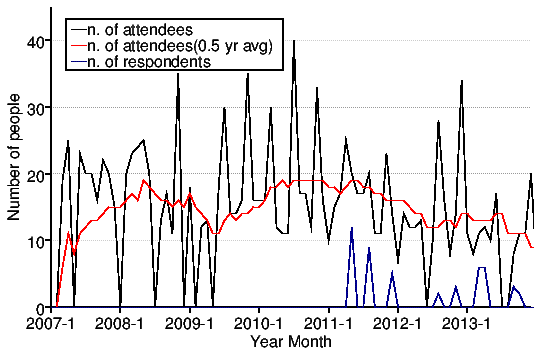
\includegraphics[width=.6\hsize]{image201312/memberanalysis/kansai.png}
    \end{center}
  \end{figure}
\end{frame}

\begin{frame}
  \frametitle{今年のイベント/お題}
  \begin{itemize}
  \item \color[rgb]{1,0,0}{月刊Debian Policy, GNOMEネタ}
  \item \color[rgb]{0,0,1}{コミュニティ}
    \begin{itemize}
    \item Using Drupal on Debian, Debian Installerトラブルシューティング,
      UbuntuとGNOME Shellと私, Linuxとサウンドシステム, ALSAのユーザーランド解説
    \end{itemize}
  \item \color[rgb]{0,.5,.5}{イベント}
    \begin{itemize}
    \item 大統一Debian勉強会, OSC 2013 Kansai@Kyoto, KOF 2013
    \end{itemize}
  \end{itemize}
\end{frame}


\takahashi[50]{月刊?\\Debian Policy}
\begin{frame}
  \frametitle{月刊Debian Policy}
  一回しかでけんかった。。。
\end{frame}

\begin{frame}
  \frametitle{GNOMEネタ}
  \begin{description}
  \item[発端]\mbox{~}\\
    wheezyでGNOME3になる
  \item[目的]\mbox{~}\\
    \begin{itemize}
    \item
      GNOME3でどう変わっているのかを学ぶ
    \item
      Debian初心者に説明、質問に答えられるようになる
    \end{itemize}
  \item[現状]\mbox{~}\\
    \begin{itemize}
    \item 説明できるようになるまでには。。。
    \item Jessieで標準デスクトップはどうなるんでしょうかね。
    \end{itemize}
  \end{description}
\end{frame}

\begin{frame}
  \frametitle{コミュニティ}
  \begin{description}
  \item[Drupal] \mbox{~}\\

    紀野さん「Using Drupal on Debian」
  \item[GREE] \mbox{~}\\

    Yuryu さん「Debian Installerトラブルシューティング」
  \item[Ubuntu Japanese Team] \mbox{~}\\

    いくやさん「UbuntuとGNOME Shellと私」

    坂本さん「Linuxとサウンドシステム」「ALSAのユーザーランド解説」
  \item[GNOMEプロジェクト] \mbox{~}\\

    松澤さん
  \end{description}
\end{frame}

\begin{frame}
  \frametitle{定例ネタ(パッケージ作成, バグ報告など)}
  \begin{exampleblock}{背景・目的}
    {\small{
        2007年度から関西でも Debian 勉強会を始動しています。
        \alert{短期的な目標は、Debian Developer(Debian開発者,以下DD) を増やすことです。}
        東京ではDebian勉強会が開催されてきましたが、一方の関西は、東京にくらべて DD の数が少ないです。 関西 Debian 勉強会は、DD と出会って GPG Key Sign をするチャンスを提供します。 また、勉強会を行うことを通して、Debian に関する知識を共有します。}}
    \vskip.5em
    \hspace*\fill{\small--- http://wiki.debian.org/KansaiDebianMeeting}
  \end{exampleblock}
  \begin{itemize}
  \item
    リリースノートを読んでみよう。、Debianの歩き方、git-buildpackage入門again
    \begin{itemize}
    \item \alert{少なかった?}
    \end{itemize}
  \item NM プロセス中 -- 2名(佐々木, 倉敷さん)
  \item DD 以外での貢献
  \end{itemize}
\end{frame}

\takahashi[50]{大いなる\\反省点}
\takahashi[100]{今年も}
\takahashi[150]{運営}

\takahashi[25]{運営フロー、ネタの見直し}

\begin{frame}
  \frametitle{イベント}
  \begin{itemize}
  \item 定例は以下の通り
    \begin{description}
    \item[OSC Kansai@Kyoto] \mbox{~}\\
      来年も8月
    \item[KOF 2014] \mbox{~}\\
      来年も11月
    \item[大統一Debian勉強会] \mbox{~}\\
      来年は長野?
    \end{description}
  \item 課題:
    \begin{itemize}
    \item ブース展示をどうするか?
    \end{itemize}
  \end{itemize}
\end{frame}

\takahashi[50]{2014年の企画}

\begin{frame}
  \frametitle{2014年の企画}
\end{frame}

\takahashi[50]{そんな\\こんなで}
\takahashi[50]{来年も頑張りましょう}

\takahashi[120]{次}

\section{今後の予定}
\begin{frame}[fragile]
\frametitle{今後の予定}

\begin{block}{第80回関西Debian勉強会}
  \begin{itemize}
  \item 日時: 1月26日(日) 13:30 -
  \item 会場: 港区民センター?
  \end{itemize}
\end{block}

\begin{block}{第108回東京エリアDebian勉強会}
  \begin{itemize}
  \item 日時: 1月18日(土)
  \item 会場、内容は調整中
  \end{itemize}
\end{block}

\end{frame}

\takahashi[50]{  }

\end{document}
%%% Local Variables:
%%% mode: japanese-latex
%%% TeX-master: t
%%% End:
